\subsection{Parte 1}



%%%%%%%%%%%%%%%%%%%%%%%%%%%%%%%%%%%%%%%%%%%%%%
%%%%%%%%%%%%%%%%%%%%%%%%%%%%%%%%%%%%%%%%%%%%%%
\subsubsection{Condensatori}

\paragraph{Modelli parametrici stimati}

La misura dell'impendenza prevede il posizionamento delle sonde dell'oscilloscopio ai capi delle componenti da misurare, il modello conseguente per la capacità è perciò $ Z = \tfrac{1}{jwC} $.

%Si reputa tuttavia impossibile eliminare ogni resistenza, %anche solo per la presenza dei collegamenti o di componenti %incognite interne all'oscilloscopio stesso, che per quanto %piccole, si vuole darne conferma o rigetto su base empirica.

%Il modello utilizzato per la stima dell'impedenza della %capacità ammette perciò la presenza di una componente %resistiva parassita incognita  $ R_{p} $.

%Da una stima preliminare e dall'analisi dell'andamento delle %fasi dell'impendenza, risulta scartata a priori l'ipotesi, %più probabile, che tali resistenze parassite possano %presentarsi in parallelo: in tal caso infatti l'andamento %della fase dovrebbe essere decrescente, cosa che non viene %osservata. L'impedenza sarebbe infatti
%\begin{align}
%\frac{1}{Z} = \frac{1}{R_{p}} + jwC
%\end{align}

%Adottando perciò l'ipotesi residuale di eventuali resistenze %parassite in serie, l'impedenza risulta $ Z = R_{p} + %\tfrac{1}{jwC} $ e perciò

$$ |Z| = \frac{1}{(\omega C)^2}$$
$$ arg Z = - \pi/2, \quad \theta = CR_{p} $$

%Dal modulo dell'impendenza si ricavano sia $ R_{p} $ che la %capacità $C$, mentre dall'argomento risulta identificabile %solo il loro prodotto
%$ \theta = CR_{p} $.
%In particolare, il modello per il modulo permette di testare %l'ipotesi di $R_{p}$ nulla, includendo il modello minimale %di assenza di resistenza $R_{p}$.


%%%%%%%%%%%%%%%%%

Per quanto riguarda la funzione di trasferimento, il parametro oggetto di stima è il prodotto $ \gamma = CR_{t} $, dove $ R_{t} $ è la resistenza totale del circuito

$$ |H| = ( 1 + (w\gamma)^{2} )^{-\frac{1}{2}} $$
$$ arg H = \arctan( -w\gamma ), \quad \gamma = CR_{t}$$


\paragraph{Dati} $ |Z| $ è il rapporto della differenza di potenziale $  V_{b-a} $ con la corrente misurata come $ V_{b} / R_{tot} $. In $ R_{tot} $ si tiene conto sia del resistore nel circuito, che della resistenza interna del generatore 
$ R_{t} = (14870 + 50) $ $\pm 1\%$.

\break
\paragraph{Risultati e commenti}
%
Relativamente alle componenti da $11$ $nF$ e $15$ $k\Omega$, la stima del valore di $C$ è compatibile con il valore di riferimento, così come l'intercetta del grafico dell'argomento è in linea con le aspettative.\\
%
In merito al grafico e alle stime dell'argomento dell'impedenza si osserva però che il modello utilizzato vincola un andamento rettilineo. La serie dei dati potrebbe essere però ben fittata anche da una curva crescente con le frequenze, evidenza compatibile con una resistenza parassita in serie con la capacità. La verifica è stata fatta adattando ai dati di impendeza un modello che comprende una resistenza in serie,  fondato sull'argomento che sia impossibile nella pratica eliminare ogni resistenza, anche solo per la presenza dei collegamenti o di componenti incognite interne all'oscilloscopio stesso, per quanto piccole. Di tale verifica non riportiamo i risultati perchè dai fit ottenuti la resistenza non viene rilevata nei dati relativi al modulo dell'impendenza.\\
%
Per quanto riguarda la funzione di trasferimento, i valori stimati di $C$, ricavati dividendo per la resistenza totale del circuito $15920$ $\Omega$ la media del prodotto $CR_{t}$ ottenuto dai dati del modulo e dell'argomento, risultano in buon accordo con quelli precedentemente ricavati con l'analisi dell'impedenza.\\
%
%
\begin{table}[H]
\begin{center}
\begin{tabular}{|c|c|c|c|c|c|c|c|}
\hline

\multicolumn{2}{|c|}{Misura}  & Parametro   & U.tà & Stima & $\pm$ Errore & Chi2 / NDF     \\ \hline

\multirow{ 2}{*}{Imp}
& mod & C  & $[nF]$     
& 11.4 & $\pm$    0.1 &  7 / 11    \\

& arg & $int.tta$ & - 
& -1.55 & $\pm$ 0.01 &  11 / 11      \\ \hline


\multirow{ 2}{*}{FdT}
& mod & $CR_{t}$ & $[\Omega\cdot nF]$ & 154700  & $\pm$ 1539 & 11 / 11      \\ 
& arg & $CR_{t}$ & $[\Omega\cdot nF]$ & 179500  & $\pm$  5711 &  11 / 11      \\
\multicolumn{2}{|c|}{}  & $R_{t}$ & $[\Omega]$  
& 14870 + 50  & $\pm$  150 &       \\
\multicolumn{2}{|c|}{}  & $C$ & $[nF]$  
& 11.2  & $\pm$  0.6 &       \\ \hline

\end{tabular}

\label{C3_P1_fit_cond1}

\caption{
Fit output. Condensatore 11 [nF] valore di riferimento.
}

\end{center}

\end{table}




Relativamente alle componenti da $46$ $nF$ e 677 $\Omega$, valgono conclusioni del tutto analoghe. I dati confermano inoltre che le stime parametriche ottenute dalla funzione di trasferimento sono meno precise di quelle derivanti dall'impendeza. Ciònondimeno le due analisi restituiscono risultati in accordo, tra loro, e con il valore di riferimento.


\begin{table}[H]
\begin{center}
\begin{tabular}{|c|c|c|c|c|c|c|}
\hline

\multicolumn{2}{|c|}{Misura}  & Parametro   & U.ta & Stima & $\pm$ Errore & Chi2     \\ \hline

\multirow{ 2}{*}{Imp}
& mod & C  & $[nF]$     
&   47 & $\pm$    2 &  10 / 10    \\

& arg & int.tta & - 
& -1.55 & $\pm$ 0.01 &  9 / 9      \\ \hline


\multirow{ 2}{*}{FdT}
& mod & $CR_{t}$ & $[\Omega\cdot nF]$ 
& 27630  & $\pm$ 564 & 10 / 10      \\

& arg & $CR_{t}$ & $[\Omega\cdot nF]$ 
& 34590  & $\pm$ 4574 & 10 / 10      \\

\multicolumn{2}{|c|}{}  & $R_{t}$ & $[\Omega]$  
& 677 + 50  & $\pm$  10 &       \\

\multicolumn{2}{|c|}{}  & $C$ & $[\Omega]$  
& 43  & $\pm$  4 &       \\ \hline


\end{tabular}

\label{C3_P1_fit_cond2}

\caption{
Fit output. Condensatore 46 [nF] valore di riferimento. }

\end{center}

\end{table}

La miglior stima delle due capacità risulta in conclusione essere
$$
C_{1} = 11.4 \pm 0.1 $$
$$
C_{2} = 47 \pm 2
$$

\paragraph*{Note: chi quadrato}
\label{Note Chi quadrato}

L'adattamento dei modelli teorici è stato ottenuto con fit non lineare. Diversamente da quanto avviene in un modello di regressione lineare ( ad esempio minimi quadrati non pesati), la stima dei parametri può mostrare forte dipendenza sia dalle condizioni iniziali impostate che dall'ampiezza degli errori. In questa analisi le condizioni iniziali erano ben note, sia dai valori di riferimento, sia da quelli ottenuti con multimetro palmare in fase preliminare. Per quanto riguarda invece gli errori sperimentali, abbiamo riscontrato che nella maggior parte dei fit gli errori sperimentali erano molto più grandi di quanto fosse giustificabile in base alla differenza quadratica media dei residui di regressione dai valori osservati. Per tale motivo, una volta ottenuta la prima stima, il modello è stato ristimato abbattendo gli errori sperimentali di un fattore proporzianale al rapporto tra varianza dei residui di regressione e gradi di libertà. Alla conclusione di questo capitolo si riportano le formule esatte utilizzate. In alcuni casi, questo procedimento è stato reiterato fino ad ottenere dei rapporti chi quadrato su gradi di libertà vicini all'unità.



%%%%%%%%%%%%%%%%%%%%%%%%%%%%%%%%%%%%%%%%%%%%%%
\break
\subsubsection*{Condensatore 11 nF: grafici e dati}

\begin{figure}[H]
\centering
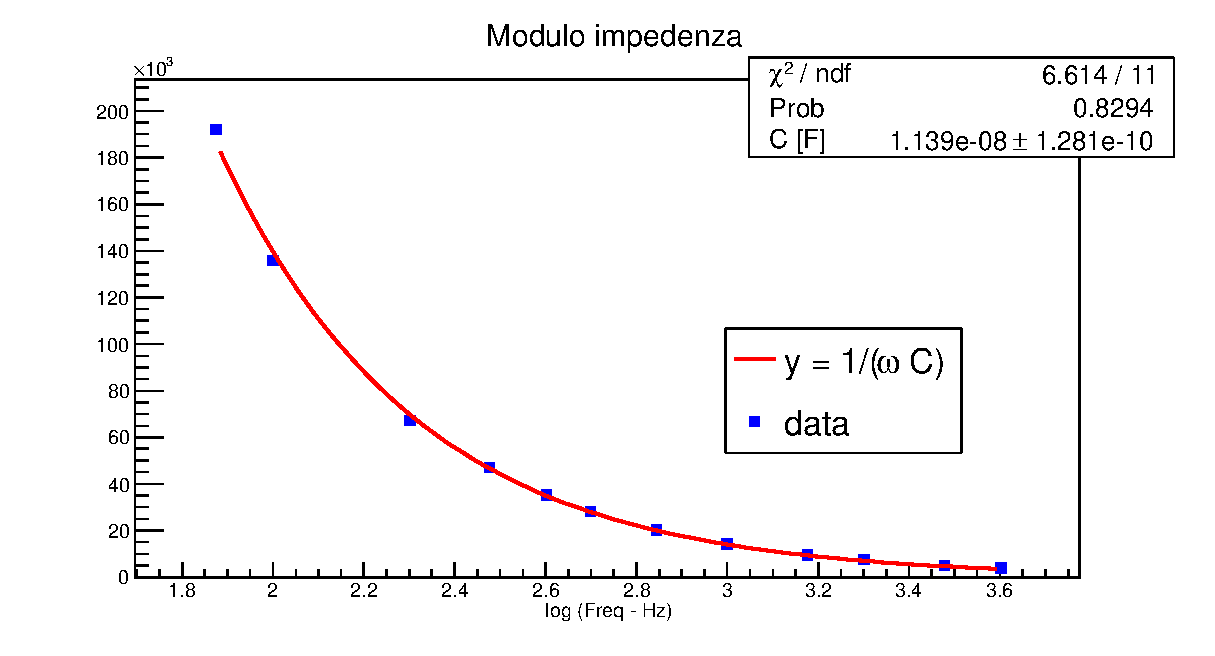
\includegraphics[scale=0.7]{Grafici/C3_P1_ModImp_cond1.eps}
\caption{
Circuito RC serie.
Ascisse [log( Freq. [Hz])].
Resistenza circuito 14870+50 [ohm]
Condensatore 11 [nF].
}
\label{fig:C3_P1_ModImp_cond1}
\end{figure}

\begin{figure}[H]
\centering
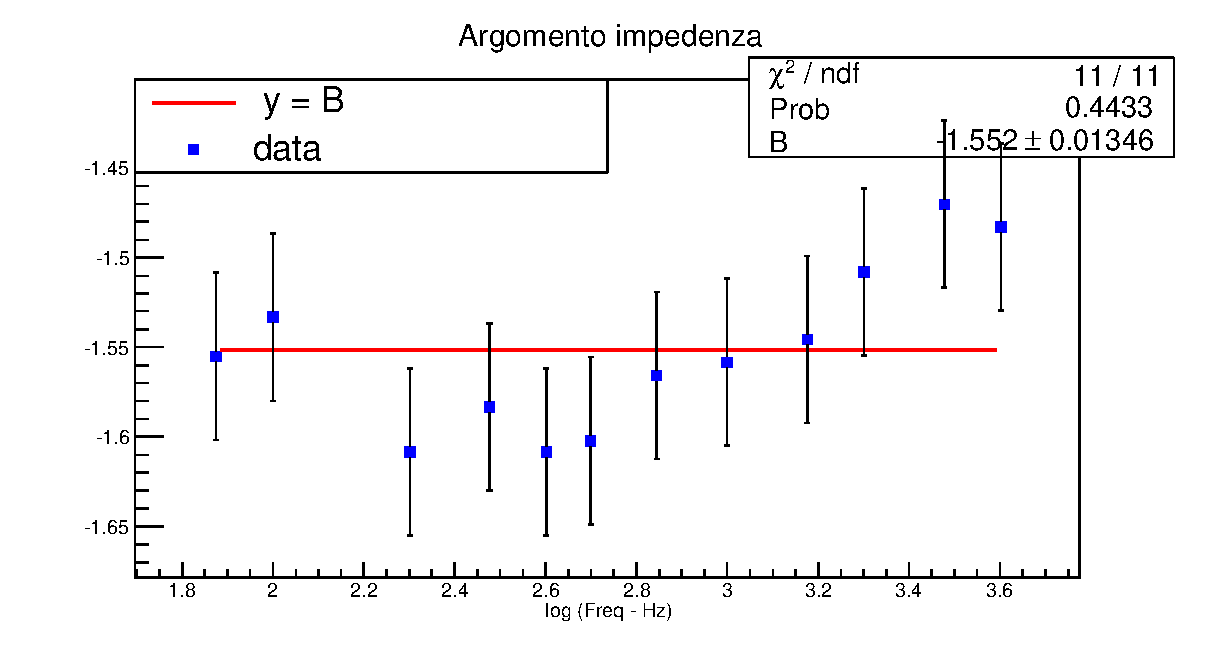
\includegraphics[scale=0.7]{Grafici/C3_P1_ArgImp_cond1.eps}
\caption{
Circuito RC serie.
Ascisse [log( Freq. [Hz])].
Resistenza circuito 14870+50 [ohm]
Condensatore 11 [nF].
}
\label{fig:C3_P1_ArgImp_cond1}
\end{figure}

\begin{figure}[H]
\centering
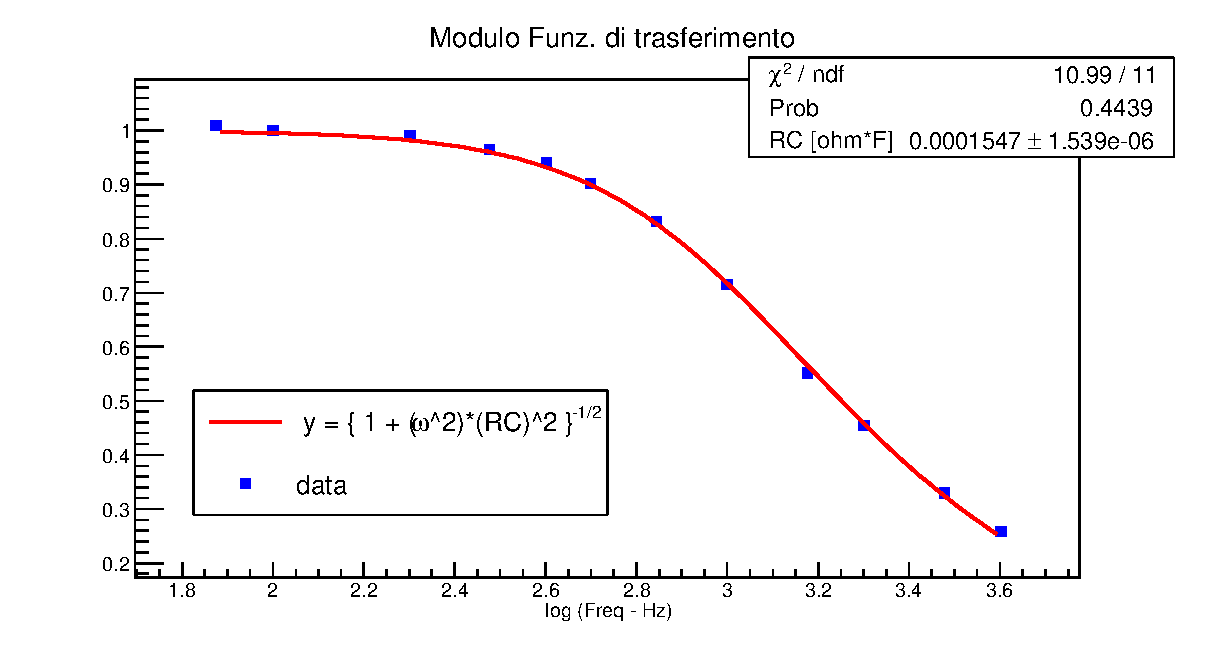
\includegraphics[scale=0.7]{Grafici/C3_P1_ModFdT_cond1.eps}
\caption{
Circuito RC serie.
Ascisse [log( Freq. [Hz])].
Resistenza circuito 14870+50 [ohm]
Condensatore 11 [nF].
}
\label{fig:C3_P1_ModFdT_cond1}
\end{figure}

\begin{figure}[H]
\centering
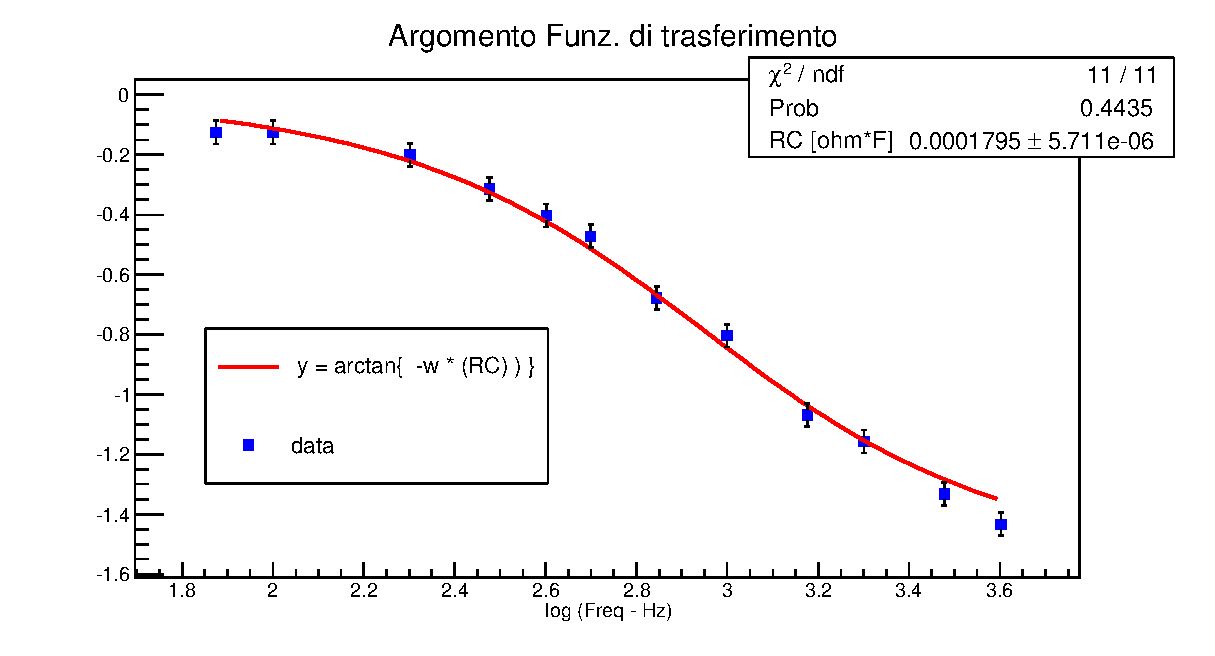
\includegraphics[scale=0.7]{Grafici/C3_P1_ArgFdT_cond1.eps}
\caption{
Circuito RC serie.
Ascisse [log( Freq. [Hz])].
Resistenza circuito 14870+50 [ohm]
Condensatore 11 [nF].
}
\label{fig:C3_P1_ArgFdT_cond1}
\end{figure}


%%%%%%%%%%%%%%%%%%%%%%%%%%%%%%%%%%%%%%%%%%%%%%
\begin{table}[H]
\begin{center}
\begin{tabular}{|r|r|r|r|r|r|r|r|}
\hline
\multicolumn{1}{|l|}{Freq} & \multicolumn{1}{l|}{Va} & \multicolumn{1}{l|}{Vb} & \multicolumn{1}{l|}{Vb-a} & \multicolumn{1}{l|}{-Fase (CH2)} & \multicolumn{1}{l|}{err-(CH2)} & \multicolumn{1}{l|}{-Fase (CH1)} & \multicolumn{1}{l|}{err-(CH1)} \\ \hline
\multicolumn{1}{|l|}{Hz} & \multicolumn{1}{l|}{V} & \multicolumn{1}{l|}{V} & \multicolumn{1}{l|}{V} & \multicolumn{1}{l|}{$\mu$s} & \multicolumn{1}{l|}{$\mu$s} & \multicolumn{1}{l|}{$\mu$s} & \multicolumn{1}{l|}{$\mu$s} \\ \hline
\multicolumn{1}{|c|}{$\pm$ 1} & \multicolumn{1}{c|}{$\pm$ 0.08} & \multicolumn{1}{c|}{$\pm$ 0.08} & \multicolumn{1}{c|}{$\pm$ 0.16} & \multicolumn{1}{l|}{} & \multicolumn{1}{c|}{$\pm$ } & \multicolumn{1}{l|}{} & \multicolumn{1}{c|}{$\pm$ } \\ \hline
75 & 10.2 & 0.80 & 10.3 & 3300 & 200 & 6400 & 200 \\ \hline
100 & 10.2 & 1.12 & 10.2 & 2,440 & 80 & 4800 & 80 \\ \hline
200 & 10.2 & 2.24 & 10.1 & 1,280 & 40 & 2340 & 40 \\ \hline
300 & 10.2 & 3.12 & 9.84 & 840 & 40 & 1500 & 40 \\ \hline
400 & 10.2 & 4.08 & 9.60 & 640 & 20 & 1090 & 20 \\ \hline
500 & 10.2 & 4.88 & 9.20 & 510 & 20 & 850 & 20 \\ \hline
700 & 10.1 & 6.16 & 8.40 & 356 & 8 & 560 & 8 \\ \hline
1000 & 10.3 & 7.68 & 7.36 & 248 & 8 & 372 & 8 \\ \hline
1500 & 10.3 & 8.88 & 5.68 & 164 & 4 & 220 & 4 \\ \hline
2000 & 10.2 & 9.36 & 4.64 & 120 & 4 & 158 & 4 \\ \hline
3000 & 10.2 & 9.92 & 3.36 & 78 & 2 & 96 & 2 \\ \hline
4000 & 10.2 & 10.0 & 2.64 & 59 & 2 & 68 & 2 \\ \hline
\end{tabular}
\end{center}
\caption{Condensatore 11 [nF]. Resistore 14.870 [ohm]}
\label{C3_P1_cond1}
\end{table}










%%%%%%%%%%%%%%%%%%%%%%%%%%%%%%%%%%%%%%%%%%%%%%
%%%%%%%%%%%%%%%%%%%%%%%%%%%%%%%%%%%%%%%%%%%%%%
\break
\subsubsection*{Condensatore 46 nF: grafici e dati}

%%%%%%%%%%%%%%%%%%%%%%%%%%%%%%%%%%%%%%%%%%%%%%
\begin{figure}[H]
\centering
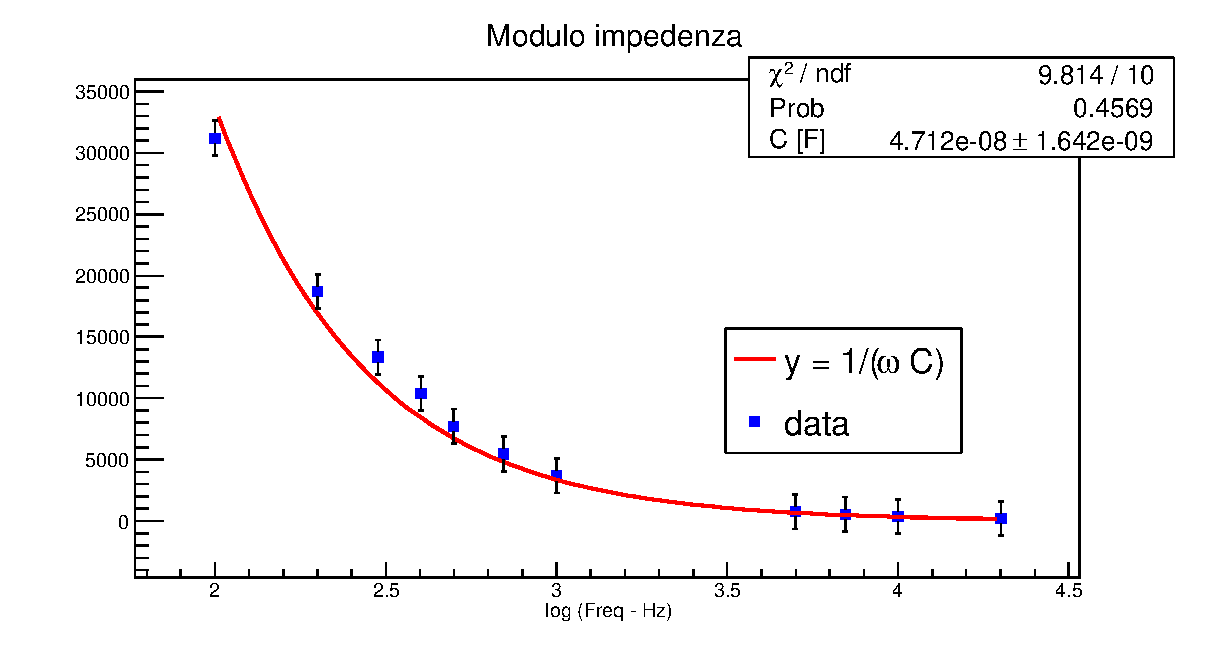
\includegraphics[scale=0.7]{Grafici/C3_P1_ModImp_cond2.eps}
\caption{
Circuito RC serie.
Ascisse [log( Freq. [Hz])].
Resistenza circuito 677+50 [ohm]
Condensatore 46 [nF].
}
\label{fig:C3_P1_ModImp_cond2}
\end{figure}

\begin{figure}[H]
\centering
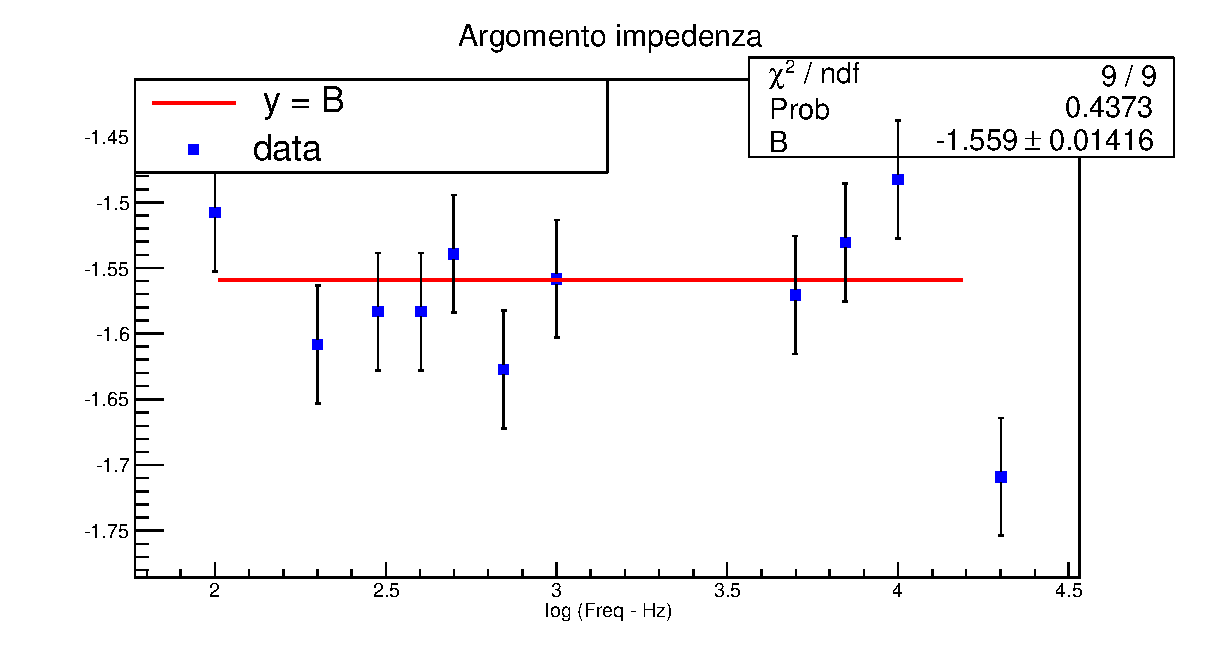
\includegraphics[scale=0.7]{Grafici/C3_P1_ArgImp_cond2.eps}
\caption{
Circuito RC serie.
Ascisse [log( Freq. [Hz])].
Resistenza circuito 677+50 [ohm]
Condensatore 46 [nF].
}
\label{fig:C3_P1_ArgImp_cond2}
\end{figure}

\begin{figure}[H]
\centering
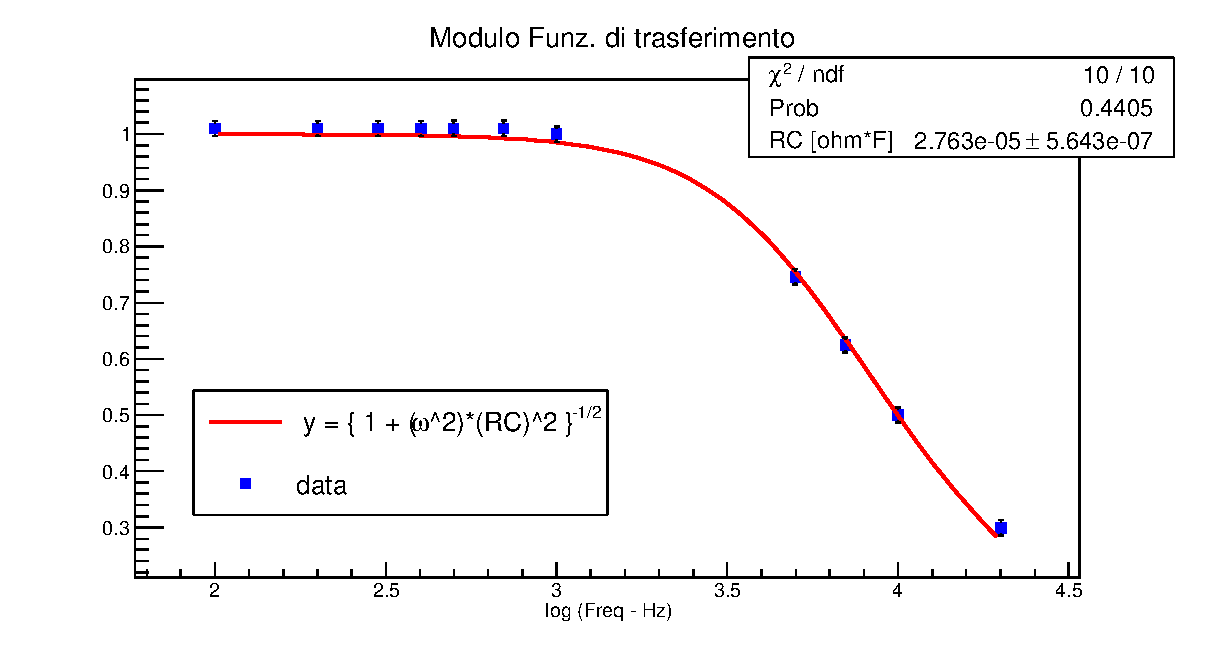
\includegraphics[scale=0.7]{Grafici/C3_P1_ModFdT_cond2.eps}
\caption{
Circuito RC serie.
Ascisse [log( Freq. [Hz])].
Resistenza circuito 677+50 [ohm]
Condensatore 46 [nF].
}
\label{fig:C3_P1_ModFdT_cond2}
\end{figure}

\begin{figure}[H]
\centering
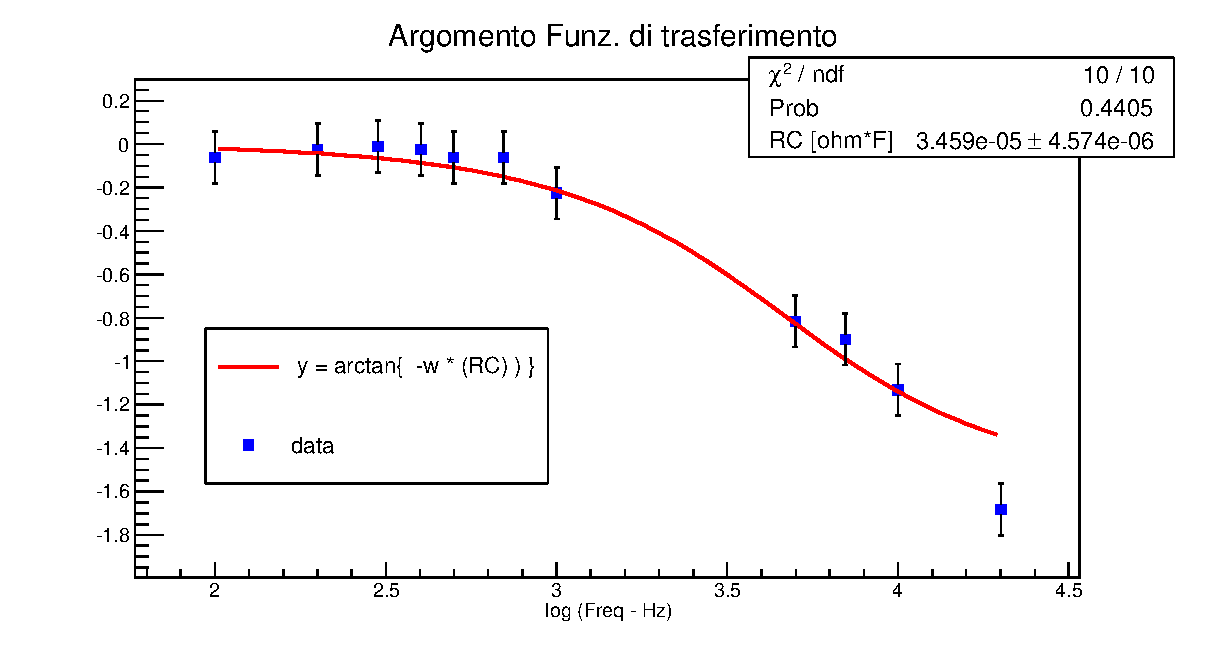
\includegraphics[scale=0.7]{Grafici/C3_P1_ArgFdT_cond2.eps}
\caption{
Circuito RC serie.
Ascisse [log( Freq. [Hz])].
Resistenza circuito 677+50 [ohm]
Condensatore 46 [nF].
}
\label{fig:C3_P1_ArgFdT_cond2}
\end{figure}


%%%%%%%%%%%%%%%%%%%%%%%%%%%%%%%%%%%%%%%%%%%%%%
\begin{table}[H]
\begin{center}
\begin{tabular}{|r|r|r|r|r|r|r|r|}
\hline
\multicolumn{1}{|l|}{Freq} & \multicolumn{1}{l|}{Va} & \multicolumn{1}{l|}{Vb} & \multicolumn{1}{l|}{Vb-a} & \multicolumn{1}{l|}{-Fase (CH2)} & \multicolumn{1}{l|}{err-(CH2)} & \multicolumn{1}{l|}{-Fase (CH1)} & \multicolumn{1}{l|}{err-(CH1)} \\ \hline
\multicolumn{1}{|l|}{Hz} & \multicolumn{1}{l|}{V} & \multicolumn{1}{l|}{V} & \multicolumn{1}{l|}{V} & \multicolumn{1}{l|}{$\mu$s} & \multicolumn{1}{l|}{$\mu$s} & \multicolumn{1}{l|}{$\mu$s} & \multicolumn{1}{l|}{$\mu$s} \\ \hline
\multicolumn{1}{|c|}{$\pm$ 1} & \multicolumn{1}{c|}{$\pm$ 0.08} & \multicolumn{1}{c|}{$\pm$ 0.08} & \multicolumn{1}{c|}{$\pm$ 0.16} & \multicolumn{1}{l|}{} & \multicolumn{1}{c|}{$\pm$ } & \multicolumn{1}{l|}{} & \multicolumn{1}{c|}{$\pm$ } \\ \hline
100 & 10.2 & 0.24 & 10.3 & 2400 & 200 & 4900 & 200 \\ \hline
200 & 10.2 & 0.40 & 10.3 & 1280 & 80 & 2480 & 80 \\ \hline
300 & 10.2 & 0.56 & 10.3 & 840 & 40 & 1660 & 40 \\ \hline
400 & 10.2 & 0.72 & 10.3 & 630 & 20 & 1240 & 20 \\ \hline
500 & 10.1 & 0.96 & 10.2 & 490 & 20 & 980 & 20 \\ \hline
700 & 10.1 & 1.36 & 10.2 & 370 & 20 & 700 & 20 \\ \hline
1000 & 10.2 & 2.00 & 10.2 & 248 & 8 & 464 & 8 \\ \hline
5000 & 9.76 & 6.88 & 7.28 & 50 & 2 & 74 & 2 \\ \hline
7000 & 9.60 & 7.92 & 6.00 & 34.8 & 0.8 & 51 & 0.8 \\ \hline
10000 & 9.44 & 8.64 & 4.72 & 23.6 & 0.8 & 32.0 & 0.8 \\ \hline
20000 & 9.36 & 9.20 & 2.80 & 13.6 & 0.4 & 11.6 & 0.4 \\ \hline
\end{tabular}
\end{center}
\caption{Condensatore 46 [nF]. Resistore 677 [ohm]}
\label{C3_P1_cond2}
\end{table}



















%%%%%%%%%%%%%%%%%%%%%%%%%%%%%%%%%%%%%%%%%%%%%%
%%%%%%%%%%%%%%%%%%%%%%%%%%%%%%%%%%%%%%%%%%%%%%
\break
\subsubsection{Induttori}

\paragraph{Modelli parametrici stimati}

A differenza dei condensatori, negli induttori si aggiunge la presenza di resistenza interna al componente stesso, l'impedenza è
$ Z = R_{p} + jwL $.


Dal modulo dell'impendenza si ricavano sia $ R_{p} $ che l'induttanza $L$, mentre dall'argomento risulta identificabile solo il loro rapporto
$ \theta = \frac{L}{R_{p}} $.

$$
|Z| = \sqrt{ R_{p}^2+ (Lw)^{2} }$$
$$
arg Z = \arctan( w\theta ), \quad \theta = \frac{L}{R_{p}}
$$



Per quanto riguarda la funzione di trasferimento, si tratta invece della resistenza totale del circuito $R_{t}$, che comprende quella del generatore e quella interna dell'induttore.

$$
|H| =   \frac{wL}{\sqrt{ R_{t}^{2} + (wL)^{2} } } 
$$
$$
arg H = \arctan( \frac{1}{w\gamma} ) \quad \gamma = \frac{L}{R_{t}}
$$

\paragraph{Dati} $ |Z| $ è il rapporto della differenza di potenziale $  V_{b-a} $ con la corrente misurata come $ V_{b} / R_{tot} $. In $ R_{tot} $ si tiene conto sia del resistore nel circuito, che della resistenza interna del generatore $50$ $\Omega$, nonchè della resistenza propria dell'induttore $R_{p} = 60$ $\Omega$, come misurata con multimetro palmare:
$ R_{t} = (677 + 50 + 60 )$ $\pm 1\%$.

\break
\paragraph{Risultati e commenti}

Per quanto riguarda il primo induttore, le stime di $L$ derivanti dal modulo dell'impedenza e da quello della funzione di trasferimento sono concordi sul valore di $0.1$ $H$, ma con un risultato più preciso di tre ordini di grandezza per la prima misura.

Per quanto riguarda la stima di $ R_{p} $, i risultati ottenuti non permettono di trarre conclusioni, a causa degli errori troppo alti.


\begin{table}[H]
\begin{center}
\begin{tabular}{|c|c|c|c|c|c|c|}
\hline

\multicolumn{2}{|c|}{Misura}  & Parametro   & U.ta & Stima & $\pm$ Errore & Chi2    \\ \hline

\multirow{ 3}{*}{Imp}
& \multirow{ 2}{*}{mod} & $R_{p}$ &  $[\Omega]$    
&  211 & $\pm$ 315 & \multirow{ 2}{*}{ 4 / 4 }     \\ 

&  & L  & $[H]$     
&   0.107 & $\pm$    0.001 &      \\

& arg & $ \tfrac{L}{R_{p}} $ & $[H / \Omega]$
& 0.00155 & $\pm$ 0.00014 &  4 / 4    \\ \hline


\multirow{ 2}{*}{FdT}
& \multirow{ 2}{*}{mod}
& $L$ & $ H $     
& 0.1  & $\pm$ 1.8     & \multirow{ 2}{*}{ 4 / 4 }  \\ 

& & $R_{t}$ & $[\Omega] $ 
& 724     & $\pm$ 11760 &      \\

& arg & $ \tfrac{L}{R_{t}} $ & $ H / \Omega $ 
& 0.0003  & $\pm$  0.0002 &      \\

\multicolumn{2}{|c|}{}  & $R_{t}$ & $[\Omega]$  
& 677 + 50 + 60  & $\pm$  10 &       \\ \hline

\end{tabular}

\label{C3_P1_fit_cond1}

\caption{
Fit output primo induttore.
}

\end{center}

\end{table}

Per quanto riguarda il secondo induttore, le stime dal modulo dell'impendeza forniscono risultati tra loro coerenti. Anche in questo caso, le misure derivanti dal modulo dell'impendenza sono molto più precise rispetto a quelle derivanti dal modulo della funzione di trasferimento. 
%
Il rapporto $ L / R_{p} $ derivante dall'argomento dell'impedenza si scosta leggermente dal rapporto delle stime derivante dal modulo. La causa di questo scostamento è da attribuirsi alla maggiore dispersione dei dati osservati rispetto al modello teorico stimato.\\ 
%
Per quanto riguarda le stime derivanti dalla funzione di trasferimento, anche per questo componente, l'incertezza sulle stime non permette di trarre conclusioni.\\
%
%
\begin{table}[H]
\begin{center}
\begin{tabular}{|c|c|c|c|c|c|c|}
\hline

\multicolumn{2}{|c|}{Misura}  & Parametro   & U.ta & Stima & $\pm$ Errore & Chi2     \\ \hline

\multirow{ 3}{*}{Imp}

& \multirow{ 2}{*}{mod} & $R_{p}$ &  $[\Omega]$    
&  72 & $\pm$    11 & \multirow{ 2}{*}{ 7 / 7 } \\ 

&  & L  & $[H]$     
&   0.0451 & $\pm$    0.0002 &  \\

& arg & $ \tfrac{L}{R_{p}} $ & $[H / \Omega]$
& $79\cdot 10^{-4}$ & $\pm$ $7.2\cdot 10^{-5}$ &  8 / 8 \\ \hline


\multirow{ 2}{*}{FdT}
& \multirow{ 2}{*}{mod} 

& $L$ & $ H $     
& 0.04  & $\pm$ 0.55     & \multirow{ 2}{*}{ 7 / 7 } \\

&
& $R_{t}$ & $ H $ 
& 814     & $\pm$ 9451 &  \\ 

& arg & $ \tfrac{L}{R_{p}} $ & $ H / \Omega $ 
& 0.0001  & $\pm$  0.0002 &   8 / 8  \\ \hline

\multicolumn{2}{|c|}{}  & $R_{t}$ & $[\Omega]$  
& 677 + 50 + 60  & $\pm$  10 &      \\ \hline

\end{tabular}

\label{C3_P1_fit_cond1}

\caption{
Fit output secondo induttore.
}

\end{center}

\end{table}
%
Fatte salve le osservazioni sulla generale scarsa precisione dei risultati ottenuti per i due induttori, si considerano come stime conclusive le stime dal modulo dell'impedenza, che presentano un errore di diversi ordini di grandezza inferiore a quelle provenienti dal modulo della funzione di trasferimento. Allo stesso risultato si perverrebbe considerando uno stimatore che combina le stime dai due esperimenti mediate per la rispettiva precisione relativa.
%
\begin{align*}
L_{1} & = 0.107   \pm 0.001 \;H \\
L_{2} & = 0.0451  \pm 0.0002 \;H
\end{align*}

\paragraph*{Note: Chi quadrato}
%
Vale quanto spiegato nel paragrafo \ref{Note Chi quadrato}



%%%%%%%%%%%%%%%%%%%%%%%%%%%%%%%%%%%%%%%%%%%%%%
%%%%%%%%%%%%%%%%%%%%%%%%%%%%%%%%%%%%%%%%%%%%%%
\break
\subsubsection*{Primo Induttore}

%%%%%%%%%%%%%%%%%%%%%%%%%%%%%%%%%%%%%%%%%%%%%%
\begin{figure}[H]
\centering
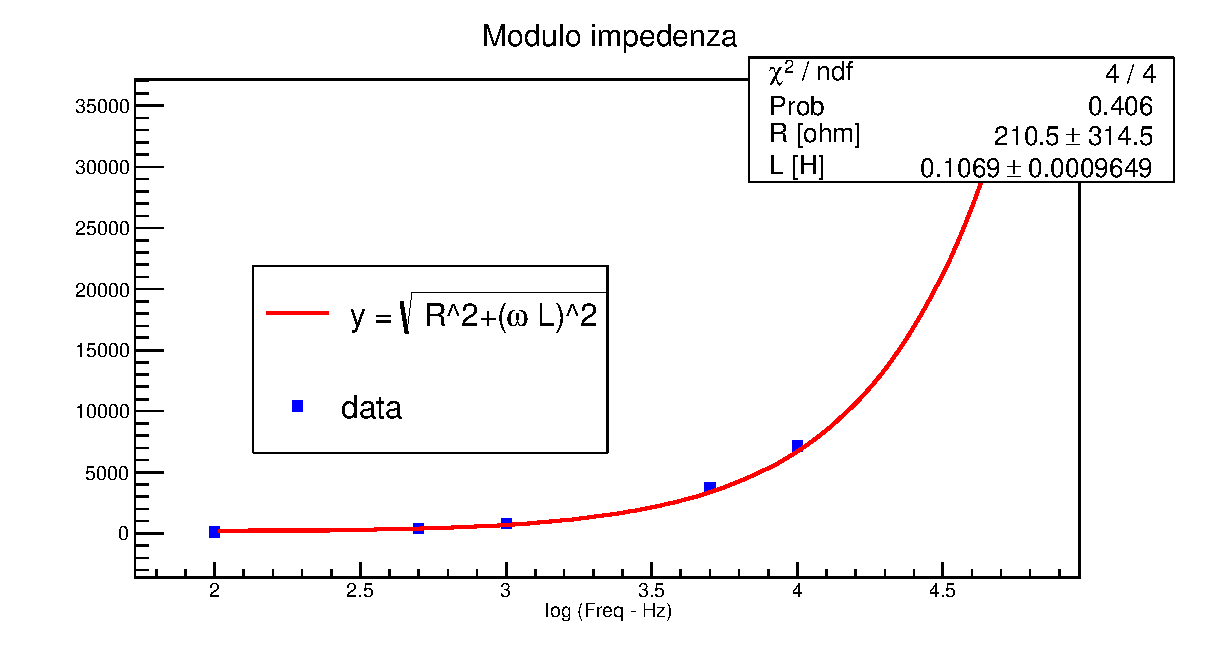
\includegraphics[scale=0.7]{Grafici/C3_P1_ModImp_ind1.eps}
\caption{
Circuito RL serie.
Ascisse [log( Freq. [Hz])].
Resistenza circuito 677+50 [ohm]
Primo induttore.
}
\label{fig:C3_P1_ModImp_ind1}
\end{figure}

\begin{figure}[H]
\centering
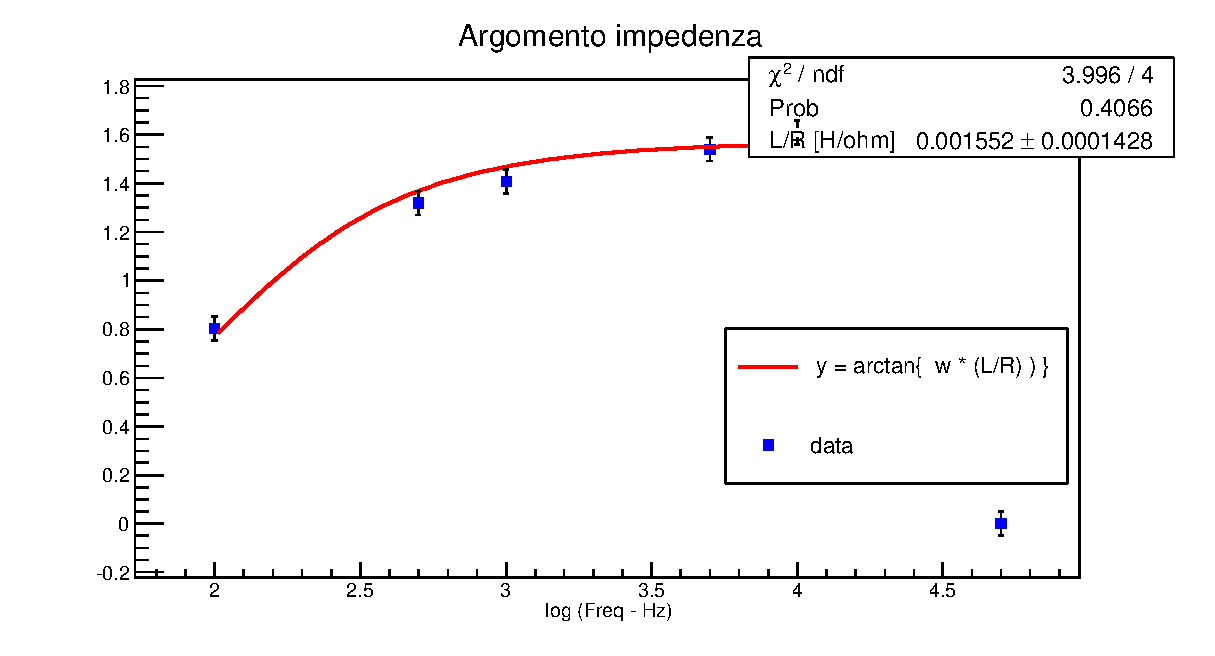
\includegraphics[scale=0.7]{Grafici/C3_P1_ArgImp_ind1.eps}
\caption{
Circuito RL serie.
Ascisse [log( Freq. [Hz])].
Resistenza circuito 677+50 [ohm]
Primo induttore.
}
\label{fig:C3_P1_ArgImp_ind1}
\end{figure}

\begin{figure}[H]
\centering
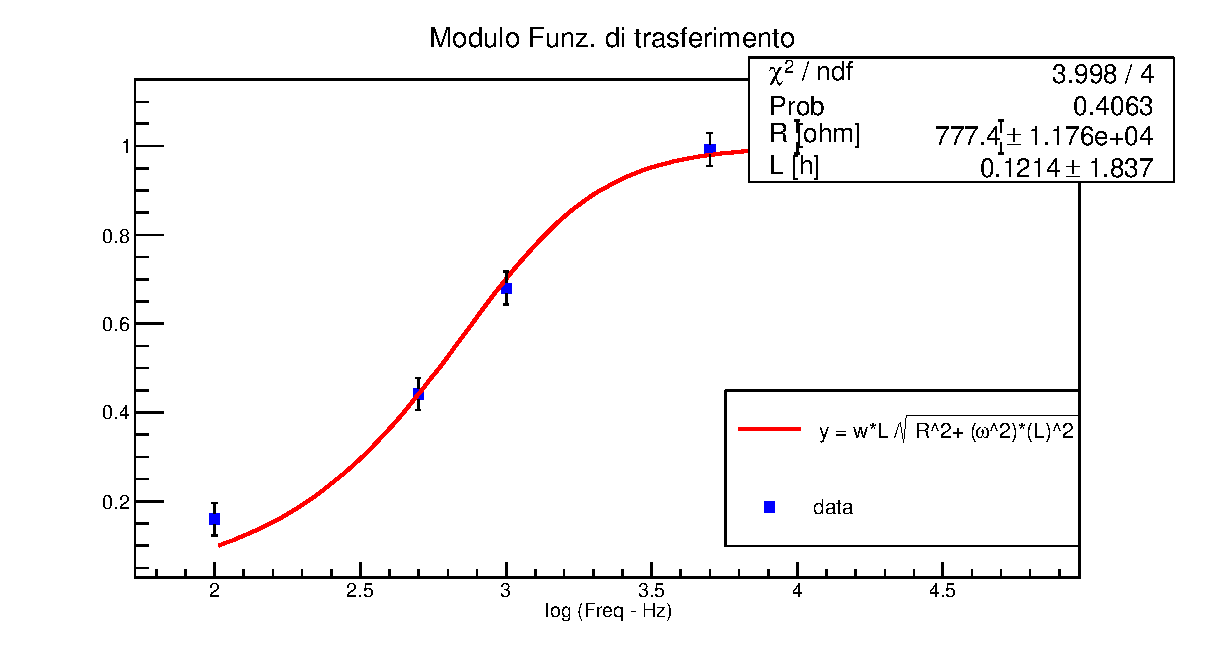
\includegraphics[scale=0.7]{Grafici/C3_P1_ModFdT_ind1.eps}
\caption{
Circuito RL serie.
Ascisse [log( Freq. [Hz])].
Resistenza circuito 677+50 [ohm]
Primo induttore.
}
\label{fig:C3_P1_ModFdT_ind1}
\end{figure}

\begin{figure}[H]
\centering
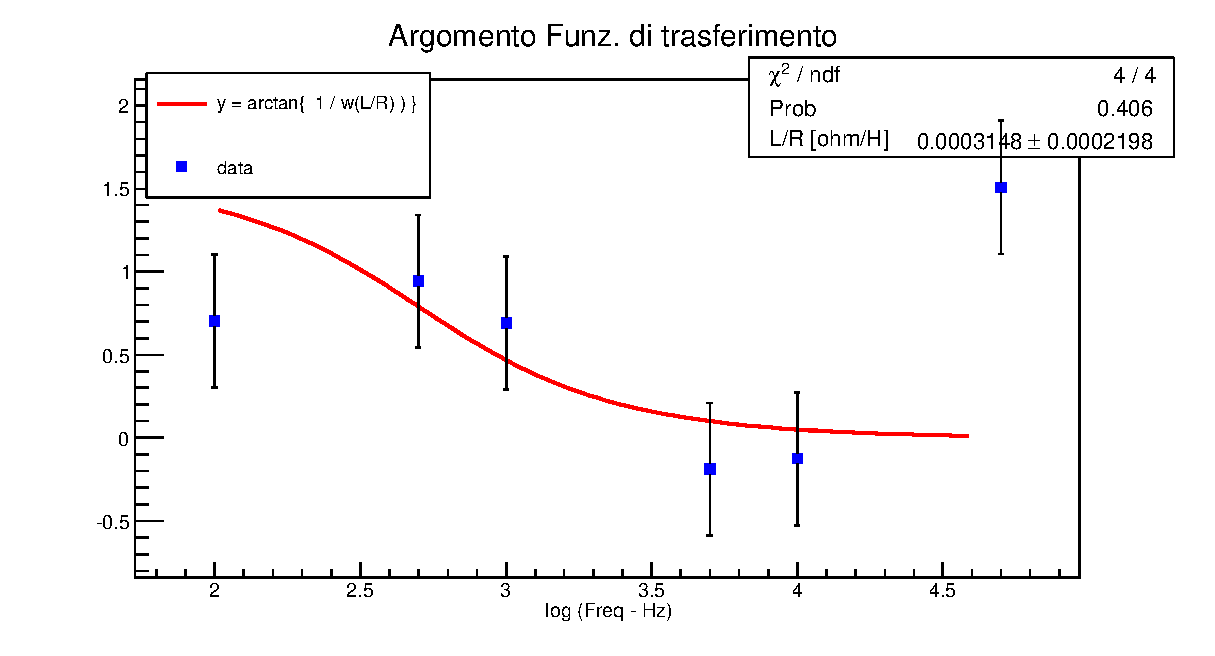
\includegraphics[scale=0.7]{Grafici/C3_P1_ArgFdT_ind1.eps}
\caption{
Circuito RL serie.
Ascisse [log( Freq. [Hz])].
Resistenza circuito 677+50 [ohm]
Primo induttore.
}
\label{fig:C3_P1_ArgFdT_ind1}
\end{figure}

\begin{table}[H]
\begin{center}
\begin{tabular}{|r|r|r|r|r|r|r|r|}
\hline
\multicolumn{1}{|l|}{Freq} & \multicolumn{1}{l|}{Va} & \multicolumn{1}{l|}{Vb} & \multicolumn{1}{l|}{Vb-a} & \multicolumn{1}{l|}{-Fase (CH2)} & \multicolumn{1}{l|}{err-(CH2)} & \multicolumn{1}{l|}{-Fase (CH1)} & \multicolumn{1}{l|}{err-(CH1)} \\ \hline
\multicolumn{1}{|l|}{Hz} & \multicolumn{1}{l|}{V} & \multicolumn{1}{l|}{V} & \multicolumn{1}{l|}{V} & \multicolumn{1}{l|}{$\mu$s} & \multicolumn{1}{l|}{$\mu$s} & \multicolumn{1}{l|}{$\mu$s} & \multicolumn{1}{l|}{$\mu$s} \\ \hline
\multicolumn{1}{|c|}{$\pm$ 1} & \multicolumn{1}{c|}{$\pm$ 0.08} & \multicolumn{1}{c|}{$\pm$ 0.08} & \multicolumn{1}{c|}{$\pm$ 0.2} & \multicolumn{1}{c|}{} & \multicolumn{1}{c|}{$\pm$ } & \multicolumn{1}{l|}{} & \multicolumn{1}{c|}{$\pm$ } \\ \hline
100 & 9.52 & 8.64 & 1.5 & 3720 & 80 & 3880 & 80 \\ \hline
500 & 9.60 & 7.92 & 4.2 & 580 & 40 & 700 & 40 \\ \hline
1000 & 9.76 & 6.56 & 6.6 & 276 & 8 & 390 & 8 \\ \hline
5000 & 10.0 & 2.08 & 9.9 & 51 & 2 & 106 & 2 \\ \hline
10000 & 10.00 & 1.12 & 10.2 & 24.4 & 0.8 & 52.0 & 0.8 \\ \hline
50000 & 10.00 & 0.24 & 10.2 & 10.0 & 0.2 & 5.2 & 0.2 \\ \hline
\end{tabular}
\end{center}
\caption{Primo induttore. Resistore 677 [ohm]}
\label{C3_P1_ind1}
\end{table}



%%%%%%%%%%%%%%%%%%%%%%%%%%%%%%%%%%%%%%%%%%%%%%
%%%%%%%%%%%%%%%%%%%%%%%%%%%%%%%%%%%%%%%%%%%%%%
\break
\subsubsection*{Secondo Induttore}

%%%%%%%%%%%%%%%%%%%%%%%%%%%%%%%%%%%%%%%%%%%%%%
\begin{figure}[H]
\centering
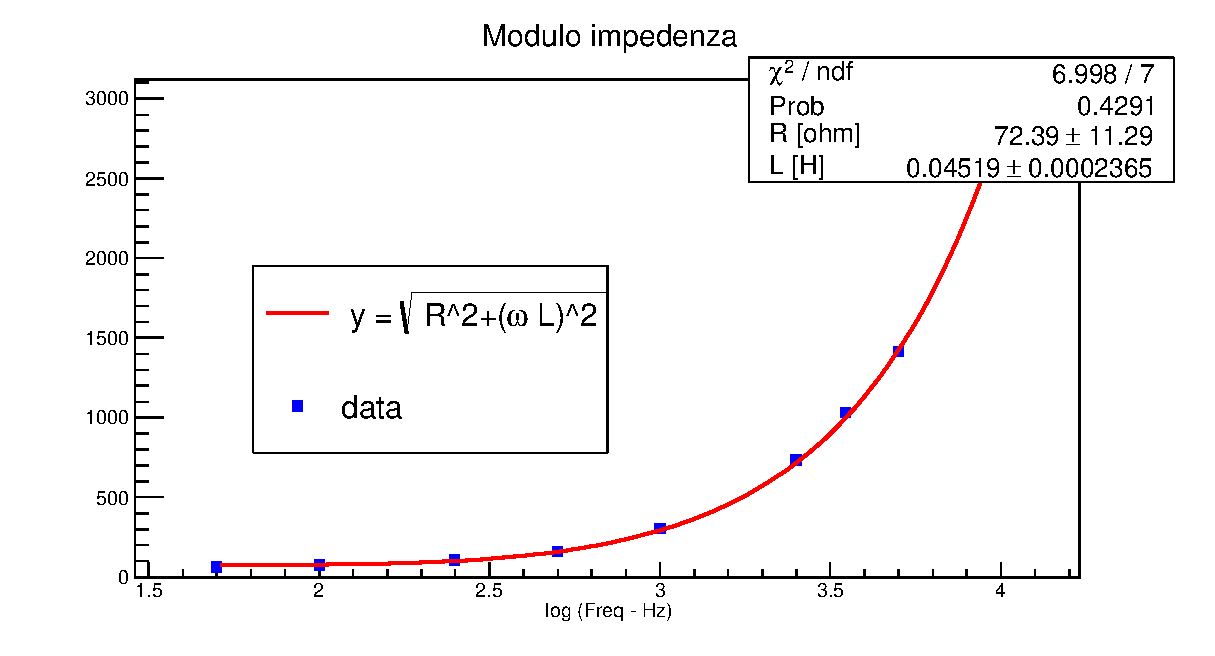
\includegraphics[scale=0.7]{Grafici/C3_P1_ModImp_ind2.eps}
\caption{
Circuito RL serie.
Ascisse [log( Freq. [Hz])].
Resistenza circuito 677+50 [ohm]
Secondo induttore.
}
\label{fig:C3_P1_ModImp_ind2}
\end{figure}

\begin{figure}[H]
\centering
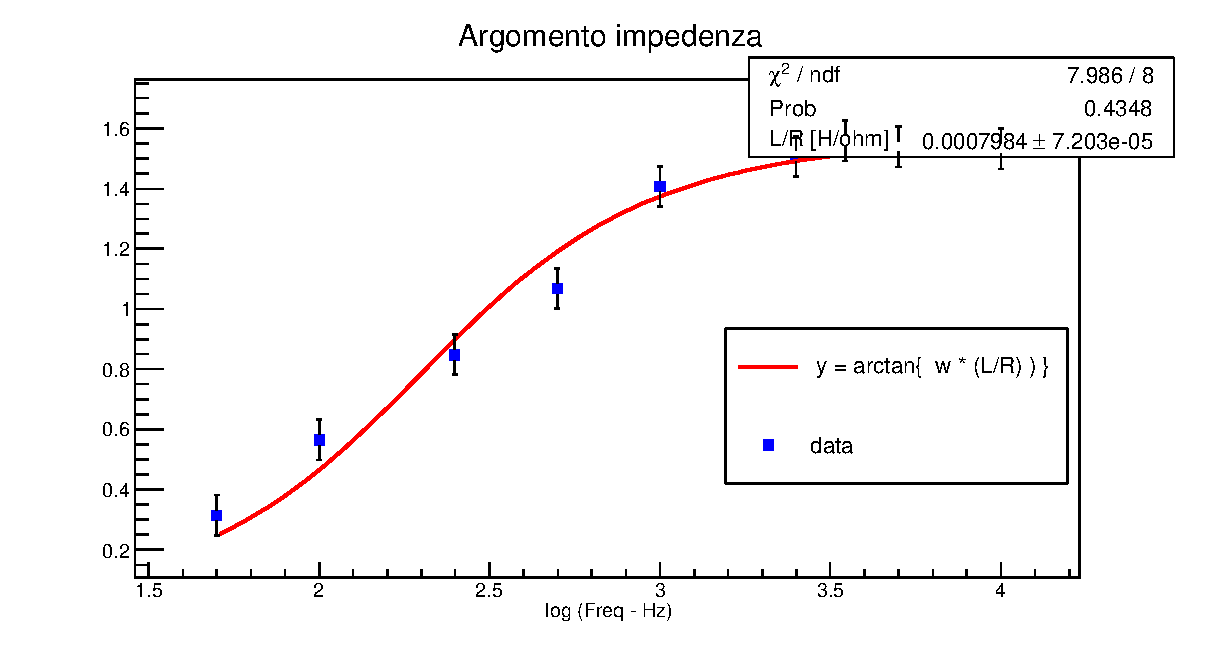
\includegraphics[scale=0.7]{Grafici/C3_P1_ArgImp_ind2.eps}
\caption{
Circuito RL serie.
Ascisse [log( Freq. [Hz])].
Resistenza circuito 677+50 [ohm]
Secondo induttore.
}
\label{fig:C3_P1_ArgImp_ind2}
\end{figure}

\begin{figure}[H]
\centering
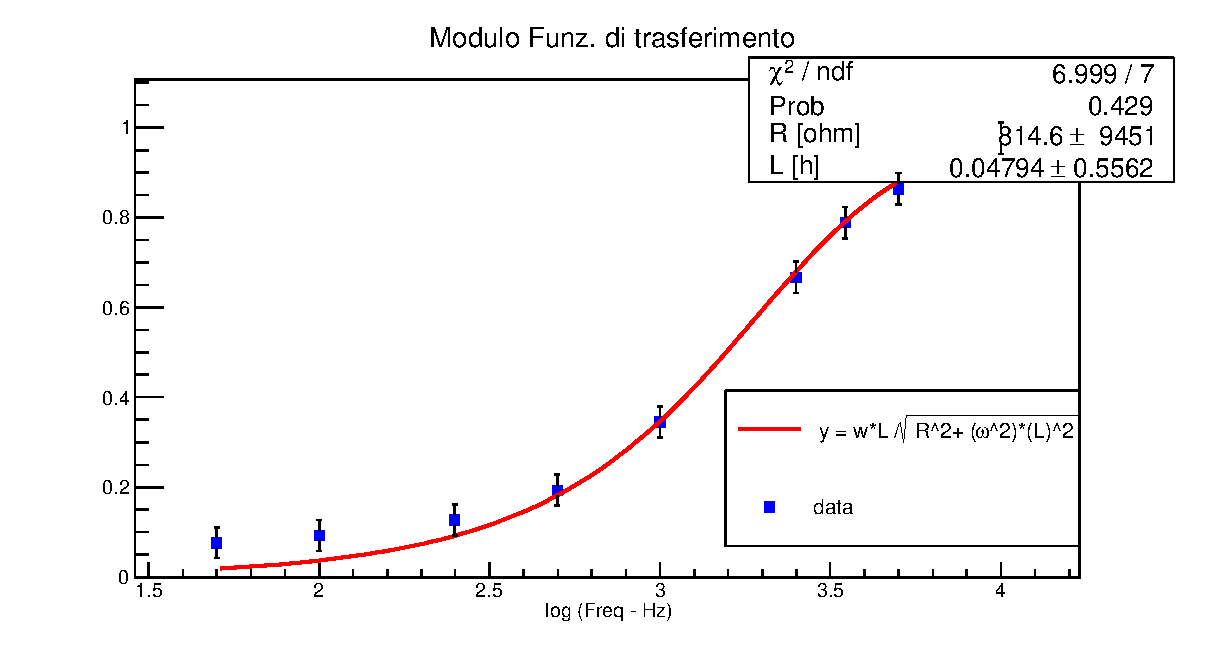
\includegraphics[scale=0.7]{Grafici/C3_P1_ModFdT_ind2.eps}
\caption{
Circuito RL serie.
Ascisse [log( Freq. [Hz])].
Resistenza circuito 677+50 [ohm]
Secondo induttore.
}
\label{fig:C3_P1_ModFdT_ind2}
\end{figure}

\begin{figure}[H]
\centering
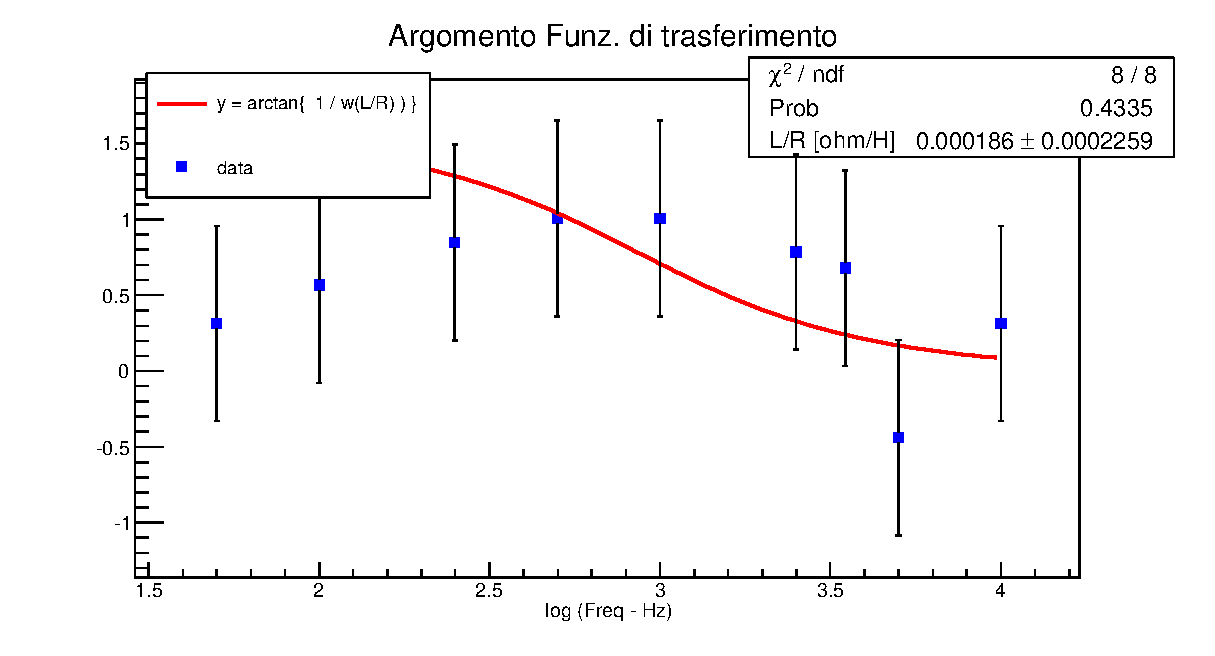
\includegraphics[scale=0.7]{Grafici/C3_P1_ArgFdT_ind2.eps}
\caption{
Circuito RL serie.
Ascisse [log( Freq. [Hz])].
Resistenza circuito 677+50 [ohm]
Secondo induttore.
}
\label{fig:C3_P1_ArgFdT_ind2}
\end{figure}

\begin{table}[H]
\begin{center}
\begin{tabular}{|r|r|r|r|r|r|r|r|}
\hline
\multicolumn{1}{|l|}{Freq} & \multicolumn{1}{l|}{Va} & \multicolumn{1}{l|}{Vb} & \multicolumn{1}{l|}{Vb-a} & \multicolumn{1}{l|}{-Fase (CH2)} & \multicolumn{1}{l|}{err-(CH2)} & \multicolumn{1}{l|}{-Fase (CH1)} & \multicolumn{1}{l|}{err-(CH1)} \\ \hline
\multicolumn{1}{|l|}{Hz} & \multicolumn{1}{l|}{V} & \multicolumn{1}{l|}{V} & \multicolumn{1}{l|}{V} & \multicolumn{1}{l|}{$\mu$s} & \multicolumn{1}{l|}{$\mu$s} & \multicolumn{1}{l|}{$\mu$s} & \multicolumn{1}{l|}{$\mu$s} \\ \hline
\multicolumn{1}{|c|}{$\pm$ 1} & \multicolumn{1}{c|}{$\pm$ 0.08} & \multicolumn{1}{c|}{$\pm$ 0.08} & \multicolumn{1}{c|}{$\pm$ 0.2} & \multicolumn{1}{l|}{} & \multicolumn{1}{c|}{$\pm$ } & \multicolumn{1}{l|}{} & \multicolumn{1}{c|}{$\pm$ } \\ \hline
50 & 9.44 & 9.04 & 0.72& 9000 & 400 & 9000 & 400 \\ \hline
100 & 9.52 & 9.04 & 0.9 & 4100 & 80 & 4100 & 80 \\ \hline
250 & 9.44 & 8.88 & 1.2 & 1460 & 40 & 1460 & 40 \\ \hline
500 & 9.52 & 8.88 & 1.8 & 660 & 40 & 680 & 40 \\ \hline
1000 & 9.52 & 8.48 & 3.3 & 276 & 8 & 340 & 8 \\ \hline
2500 & 9.84 & 7.04 & 6.6 & 104 & 4 & 150 & 4 \\ \hline
3500 & 9.84 & 5.92 & 7.8 & 72 & 4 & 112 & 4 \\ \hline
5000 & 10.0 & 4.80 & 8.6 & 51 & 2 & 114 & 2 \\ \hline
10000 & 10.0 & 2.72 & 9.8 & 25.6 & 0.8 & 45.0 & 0.8 \\ \hline
\end{tabular}
\end{center}
\caption{Secondo induttore. Resistore 677 [ohm]}
\label{C3_P1_ind2}
\end{table}